\chapter{Resultats}
\label{c:Resultats}
\fbox{\emph{\textbf{\parbox{0.9\linewidth}{
Hem de tenir en compte de que les notes finals dels alumnes estan arrodonides, per tant considerarem que la predicció ha estat encertada si té un marge d'error menor a 0,5.}}}}
\section{Resultats de la xarxa neuronal en fulls de càlculs}
Desprès de finalitzar totes les etapes, els pesos s'han ajustat correctament i, encara que l'error no s'hagi pogut aproximar-se molt al zero absolut, ja és un valor molt petit que podem donar per bo. En la seguent figura podem veure els valors dels pesos finals del model.\\

\begin{figure}[H]
    \centering
    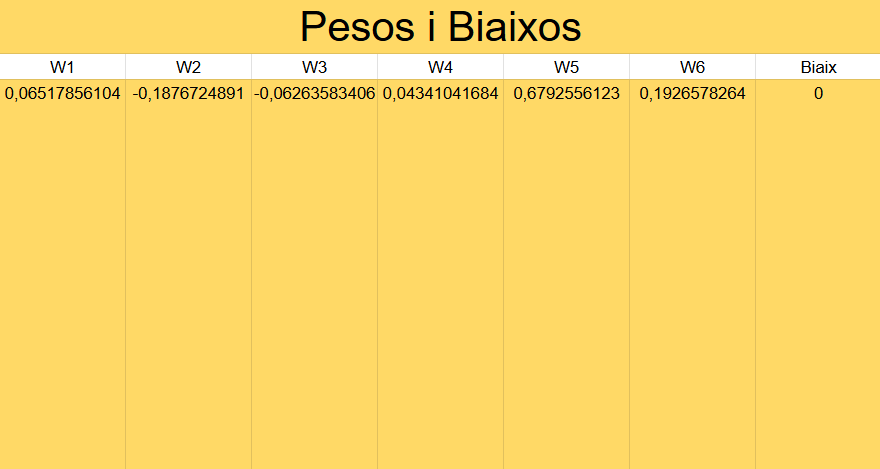
\includegraphics[width=0.5\textwidth]{./figures/Pesos_finals.png}
    \caption{Pesos finals del model}
\end{figure}

Amb aquests pesos, el model hauria de ser capaç d'obtenir unes prediccions precises respecte a la nota final dels alumnes, per obtenir els valors finals de la predicció, hem de convertir els valors normalitzats de la columna de la predicció de Y de l'última etapa en valors normals, aïllant en la mateixa fòrmula que vam emprar per normalitzar les dades.\\
$z = \frac{x - \mu}{\sigma}$\\

\begin{figure}[H]
    \centering
    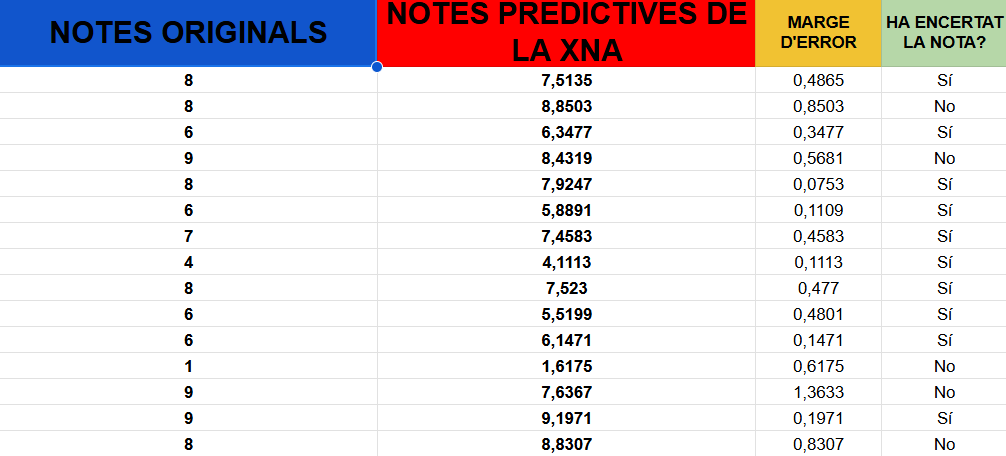
\includegraphics[width=0.5\textwidth]{./figures/Resultat_final.png}
    \caption{Prediccions finals de la pràctica}
\end{figure}

En la figura d'adalt, desprès de desnormalitzar els valors, he organitzat les notes inicials i les prediccions finals en unes taules per visualitzar-los millor, a un costat tenim les notes originals i per l'altre les predictives.
 Això ens dona que la xarxa neuronal ha encertat 10 notes de 15, per tant té una precisió aproximada del 66,7 percent.

\section{Comparació entre una xarxa neurnal creada per un llenguatge de programació netre una de fulls de calculs}
En aquest capítol, desprès de que cadascún de nosaltras haguèssim acabat les nostres respectives pràctiques, compararem els nostres resultats finals i veurem quina de les 2 formes és millor.\\

La principal diferencia que destaca entre aquests dues metodes de desenvolupament es la automatizació de l'aprenentatge (\textbf{Automatic machine}. En el cas dels fulls de càlcul, cal optimitzar i ajustar-ho tot manualment, cosa que esdevé un procés molt laboriós. En canvi, amb el llenguatge de programació, la XNA te'l fa tot el procés manual. Tanmateix, els fulls de calculs ho té tot més visual, permetent a l'usuari veure tot el treball, però en Python està oculta.\\
\begin{comment}
Per altre banda, en Python s'han utilitzat 18 enquestes y ha obtingut un resultat de 94,44\% de precisió, es a dir, ha encertat 17 notes de 18, per altre banda, el full de càlcul ha calgut de 15 enquestes y ha obtingut un 66,67\%, concretament ha encertat 10 de 15.

Podem observar que Python té una clara superioritat respecte als fulls de càlcul ja que té molta més precisió i ,a més, ha predit més notes. No obstant això, qualsevol persona que hagi fet una mica d'estadística pot manipular facilment un full de càcul, i hem de tenir en compte en que és molt més difícil fer la xarxa en Python perquè requereix de coneixements de programació.
\end{comment}

Per altre banda, la precisió de la predicció també és un factor molt important, en el nostre cas amb un full de calculs, de les 15 enquestes predictes, ha hagut una precisió de 66,67\%, en quan en Python s'ha obtingut una precisió de 94,44\%. Com podem observar la presició del python té una superioritat absoluta respecte el full de calculs, a més, amb Python ha predit més notes matematiques.\\

Un altre factor terciarí, és la corba d'aprenentatge de cadascún. Per poder fer l'ús del Python t'hauries d'aprendre el llenguatge i les seves logiques;per contra, un full de calculs pot ser manipulat perfectament per qualsevol persona que hagi cursat estadistica.


En conclusió, si volguèssim una xarxa neuronal amb la màxima presició possible, Python seria una molt bona opció, però si no vols o no tens temps d'apendre un llenguatge de programació, és millor un full de càlcul, però s'ha de tenir en compte de que te molta menys precisió.






















